\documentclass{beamer}

% -- Theme ---------------------------------------------------------------------

\usetheme[backgroundimagefile=images/bg-light,useblacktitletext,opacity=0]{diepen}
\useinnertheme{circles}
\setbeamercolor{item}{fg=black}
\setbeamercolor{structure}{fg=black}

% Alternatively:
%\usetheme{Amsterdam}

% -- Required packages ---------------------------------------------------------

\usepackage{graphics}
\usepackage{courier}
\usepackage{listings}

\lstdefinelanguage{JavaScript}{
  keywords={typeof, new, true, false, catch, function, return, null, catch, switch, var, if, in, while, do, else, case, break},
  ndkeywords={class, export, boolean, throw, implements, import, this},
  ndkeywordstyle=\bfseries,
  comment=[l]{//},
  morecomment=[s]{/*}{*/},
  morestring=[b]',
  morestring=[b]"
}

\lstset{
        language=JavaScript,
        basicstyle=\bfseries\scriptsize\ttfamily, % use fixed-width font
        keywordstyle=\bfseries\color{red}, % bold keywords
        identifierstyle=,       % nothing happens
        commentstyle=\ttfamily\color{blue}, 
        stringstyle=\bfseries\ttfamily,  % typewriter type for strings
        showstringspaces=false, % no special string spaces
        columns=fullflexible,   % Use flexible column format (for comments)
        %backgroundcolor=\color{lightgrey},%
        %rulecolor=\color{darkgrey},%
        %frame=single,%
        %frameround=tttt,
        %framerule=0.6pt,%
        %framesep=5mm,%
        %captionpos=b,%
        %xleftmargin=5mm,%
        %xrightmargin=5mm,%
        %float,%
        %morekeywords={@Model},
        %abovecaptionskip=0pt,
        %belowskip=0pt
}

% -- Command definitions -------------------------------------------------------

\newcommand{\code}[1]{\texttt{#1}}

% -- Presentation data ---------------------------------------------------------

\mode<presentation>

\title[Tachyon Overview]{Tachyon: a Meta-circular Optimizing JavaScript Virtual Machine}

\author[Chevalier-Boisvert, Lavoie, Dufour, Feeley]
{
  Maxime~Chevalier-Boisvert \and
  Erick~Lavoie \and
  Bruno~Dufour \and
  Marc~Feeley
}

\institute[UdeM]
{
  DIRO\\
  Universit\'e de Montr\'eal, Canada
}

\date[Mozilla 2011]
{Mozilla, March 28 2011}

\begin{document}

% -- Slide ---------------------------------------------------------------------
\begin{frame}
  \titlepage
\end{frame}
% ------------------------------------------------------------------------------

% -- Slide ---------------------------------------------------------------------
%% \begin{frame}{Outline}
%%   \tableofcontents
%% \end{frame}
% ------------------------------------------------------------------------------

% -- Slide ---------------------------------------------------------------------
\begin{frame}
\frametitle{\bf Outline}

  
\includegraphics[height=0.5in]{images/tachyon-icon.png}
  \begin{minipage}[b]{3.5in}
    \begin{center}
      {\em Tachyon:~~~~~~~~~~~~~~~~~~~~~~~~~~~~~~~~~~~~~~~~~~~~~~~~~~~~~~~~~\\ a hypothetical particle that travels faster than light.} \\
      -- Oxford Dictionary
    \end{center}
  \end{minipage}

  \bigskip

  \begin{itemize}

  \item {\bf System overview} -- {\em Marc Feeley}
    \smallskip

  \item {\bf IR and optimization} -- {\em Maxime Chevalier-Boisvert}
    \smallskip

  \item {\bf Back-end, profiling and benchmarks} -- {\em Bruno Dufour}
    \smallskip

  \end{itemize}

  \bigskip
  \bigskip

  Unfortunately {\em Erick Lavoie} could not be here (responsible
  for back-end and register allocator)

\end{frame}
% ------------------------------------------------------------------------------

% -- Slide ---------------------------------------------------------------------
\begin{frame}
\frametitle{\bf Goals}

  \begin{itemize}

  \item Tachyon JS project started March 2010
    \smallskip

  \item JS is a key language with a bright future
    \smallskip

  \item 2010 JS VMs performance... {\bf We can do better!}
    \smallskip

    \bigskip

  \item Goal \#1: compiler for {\bf research on dynamic languages}
    \begin{itemize}
    \item optimistic optimization
    \item object representation / garbage collection
    \item profiling real-world applications
    \item language extensions: exact arithmetic, continuations, tail calls, exceptions, concurrency, distributed computing, Harmony,~...
    \end{itemize}
    \smallskip

  \item Goal \#2: {\bf production-quality} high-performance open-source
    JS compiler for client-side and server-side scripting

  \end{itemize}

\end{frame}
% ------------------------------------------------------------------------------

% -- Slide ---------------------------------------------------------------------
\begin{frame}
\frametitle{\bf JIT Compilation}

  \begin{itemize}

  \item JIT compilers are efficient because they
    \begin{itemize}
      \item[1.] mostly compile the program parts where speed matters
      \item[2.] {\bf adapt/specialize the program} to the run time conditions
    \end{itemize}
    \smallskip

  \item In theory, {\bf dynamic recompilation may outperform static compilation}
    \smallskip

  \item {\bf Recompilation time must be kept small}
    \begin{itemize}
    \item Avoid expensive optimizations
    \item Use hand-tuned algorithms
    \item ...
    \end{itemize}
    \smallskip

  \end{itemize}
\end{frame}
% ------------------------------------------------------------------------------

% -- Slide ---------------------------------------------------------------------
\begin{frame}
\frametitle{\bf Self-Hosting JIT Thesis}

  \begin{itemize}

  \item Our idea: {\bf dynamically recompile the JIT compiler}
    \bigskip
    \bigskip

  \item {\bf Adapts the JIT compiler to the program being compiled}
    \smallskip

  \item The cost of JIT compiler adaptation is amortized over
    {\bf repeated recompilations of the same program}
    \bigskip
    \bigskip

  \item Other self-hosting benefits:
    \begin{itemize}
      \item single runtime system (one heap, GC, I/O, ...)
      \item easy introspection and dynamic language extension
    \end{itemize}
    \smallskip

  \item We are more productive in JS than C/C++

  \end{itemize}
\end{frame}
% ------------------------------------------------------------------------------

% -- Slide ---------------------------------------------------------------------
\begin{frame}
\frametitle{\bf Current State}

  \begin{itemize}

  \item Compiler is written in a subset of JS (roughly 40 KLOC)
    \begin{itemize}
    \item parsing
    \item analysis/optimization of intermediate representation
    \item in-memory assembly and linking
    \end{itemize}
    \smallskip

  \item Few extensions to the host VM (readFile, malloc, etc.)
    \smallskip

  \item Implements ES5 spec except:
    \begin{itemize}
    \item floating point (only fixnums are supported)
    \item regular expressions
    \item getters and setters, property attributes
    \item {\tt eval} and most metaprogramming features
    \item no GC yet!
    \end{itemize}
    \smallskip

  \item Back-end supports {\bf x86} and {\bf x86\_64}
    \smallskip

  \item Interactive shell since February 2011
    \smallskip

  \item Tachyon self-bootstrap achieved March 2011
    \smallskip

  \end{itemize}
\end{frame}
% ------------------------------------------------------------------------------

% -- Slide ---------------------------------------------------------------------
\begin{frame}
\frametitle{\bf Parser}

  \begin{itemize}

  \item Based on WebKit's yacc grammar
    \begin{itemize}
    \item {\tt Grammar.y} converted to LALR-SCM parser generator spec
    \item LALR-SCM tables pretty-printed as JS arrays (6 KLOC)
    \item hand written LALR driver (.3 KLOC) and scanner (1 KLOC)
    \end{itemize}
    \smallskip

  \item Parses 100 KLOC per second
    \smallskip

  \item AST keeps track of source location

  \end{itemize}

  \begin{center}
    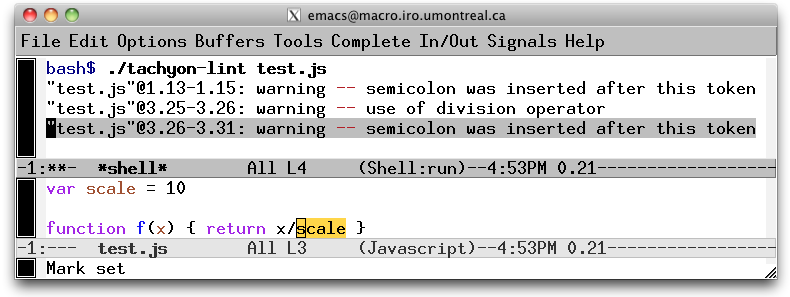
\includegraphics[height=1.5in]{images/tachyon-lint.png}
  \end{center}

\end{frame}
% ------------------------------------------------------------------------------

% -- Slide ---------------------------------------------------------------------
\begin{frame}[fragile]
\frametitle{\bf Parser Derivatives for Debugging}

  \begin{itemize}

  \item {\bf JS pretty-printer} -- dump or pretty print AST
    \smallskip

  \item {\bf js2scm} -- compile JS to Scheme
    \smallskip

  \item {\bf js2js} -- instrument JS code with function entry/exit tracing
    \smallskip

\begin{block}<+->{Execution trace of Tachyon compiler}
\begin{lstlisting}[language=]
bash$ ./js2js -debug tachyon.js > tachyon-debug.js
bash$ d8 tachyon-debug.js
|  (( "utility/iterators.js"@13.1-17.2: Iterator
|  |  (( "utility/debug.js"@73.1-77.2: assertNew
|  |  |  (( "utility/debug.js"@62.1-68.2: isGlobal
|  |  |  |  (( "utility/debug.js"@65.19-65.47: isGlobal
|  |  |  |  )) "utility/debug.js"@65.33-65.45: isGlobal
|  |  |  )) "utility/debug.js"@67.5-67.27: isGlobal
|  |  )) "utility/debug.js"@73.1-77.2: assertNew
|  )) "utility/iterators.js"@16.5-16.17: Iterator
|  (( "utility/iterators.js"@13.1-17.2: Iterator
|  |  (( "utility/debug.js"@73.1-77.2: assertNew
...
\end{lstlisting}
\end{block}

  \end{itemize}

\end{frame}
% ------------------------------------------------------------------------------

% Maxime's TOC
%
% IR
% - HIR
% - IR types
% - LIR
% - IIR
%   - Annotations
%
% IR support: static definitions
% IR support: auto-generated code
% - layouts and their methods (alloc/init, accessors)
% - GC visit code
% - FFI wrappers
%
% Compilation phases
% - Present before IR?
% - Picture
%   - Parsing
%   - AST simplification/annotation
%   - AST->IR conversion
%   - IR lowering/optimization
%   - Register allocation
%   - Machine code generation
%
% Optimistic optimizations
% - Optimization issues
% - Getting rid of guards
% - Picture(s)
%   - Specialization
%   - Execution model
% - Less about type profiling?
% - Less about related work?

%
% Slide about compilation phases, with graphic
%
\begin{frame}{Compilation Phases}
\begin{center}
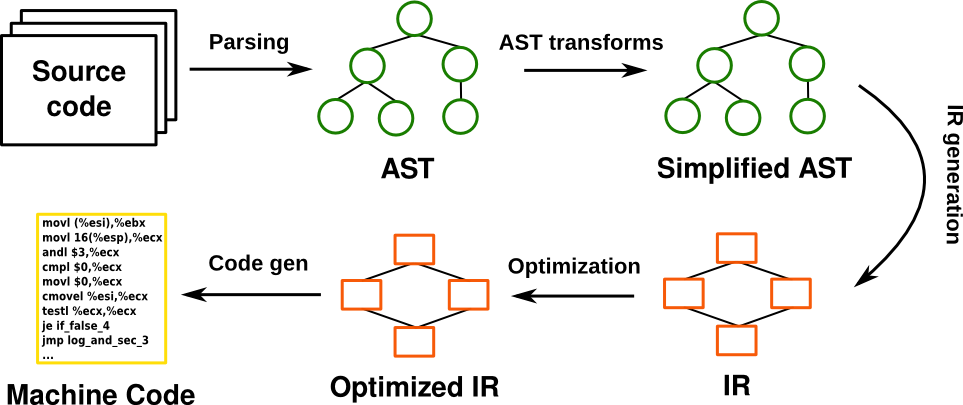
\includegraphics[width=4.5in]{images/phases}
\end{center}
\end{frame}

%
% Example of program JS->AST->HIR->LIR->ASM
%

\begin{frame}{Example: Simple Function}
\lstinputlisting{images/ex_source.js}
\end{frame}

\begin{frame}{Example: Abstract Syntax Tree}
\tiny\verbatiminput{images/ex_ast.txt}
\end{frame}

\begin{frame}{Example: High-level IR}
\tiny\verbatiminput{images/ex_hir.txt}
\end{frame}

\begin{frame}{Example: Low-level IR}
\tiny\verbatiminput{images/ex_lir.txt}
\end{frame}

\begin{frame}{Example: Machine Code}
\begin{columns}[t]

\begin{column}{0.33\textwidth}
\tiny\verbatiminput{images/ex_asm1.txt}
\end{column}

\begin{column}{0.33\textwidth}
\tiny\verbatiminput{images/ex_asm2.txt}
\end{column}

\begin{column}{0.33\textwidth}
\tiny\verbatiminput{images/ex_asm3.txt}
\end{column}

\end{columns}
\end{frame}

% -- Slide ---------------------------------------------------------------------
\begin{frame}{High-Level IR}
    \begin{itemize}

        \item Core JS semantics expressed in terms of HIR instructions
        \begin{itemize}
            \item Act on boxed, high-level (dynamic) types
            \begin{itemize}
                \item Strings, numbers, objects, \ldots
            \end{itemize}
            \item May produce exceptions in some cases
        \end{itemize}

        \item Examples
        \begin{itemize}
            \item Arithmetic/comparison operators (+, -, *, /, $<$, \ldots)
            \item Property accesses (getProp, putProp, hasProp, \ldots)
            \item Other misc. JavaScript operators (typeof, instanceof, \ldots)
        \end{itemize}

        \item Currently, HIR implemented directly by primitive functions
        \begin{itemize}
            \item Primitives written in terms of extended JS
            \item Annotated for performance
                \begin{itemize}
                    \item Static linkage, force inlining, no exceptions, etc.
                \end{itemize}
        \end{itemize}

    \end{itemize}
\end{frame}
% ------------------------------------------------------------------------------

% -- Slide ---------------------------------------------------------------------
\begin{frame}{JavaScript Extensions}
    \begin{itemize}
        \item JavaScript has no access to raw memory
        \begin{itemize}
            \item Essential to implement a VM/JIT
        \end{itemize}
        \item Tachyon is written in JS w/ “unsafe” extensions
        \begin{itemize}
            \item Minimizes the need to write C code (FFI)
            \item Maximizes performance
            \begin{itemize}
                \item FFIs are optimization boundaries
            \end{itemize}
        \end{itemize}
        \item JS code translated to low-level typed IR
        \begin{itemize}
            \item JS extensions: insert typed instructions in code as it is translated (Inline IR / IIR)
        \end{itemize}
    \end{itemize}
\end{frame}
% ------------------------------------------------------------------------------

% -- Slide ---------------------------------------------------------------------
\begin{frame}{Low-Level IR}
    \begin{itemize}
        \item Some similarities with LLVM
        \item SSA-based
        \item Type-annotated
        \begin{itemize}
            \item Integers, floats, booleans, raw pointers
            \item Boxed values, references
        \end{itemize}
        \item Low-level
        \begin{itemize}
            \item Mirrors instructions commonly found on most CPUs
            \begin{itemize}
                \item add/sub/mul/div, and/or/shift, jump/if/call, load/store, etc.
            \end{itemize}
            \item Still tries to be “machine agnostic”
            \begin{itemize}
                \item No specific endianness, no registers
            \end{itemize}
            \item Allows expressing more optimizations (specialization)
        \end{itemize}
    \end{itemize}
\end{frame}
% ------------------------------------------------------------------------------

\begin{frame}{Primitive Functions}
    \begin{itemize}
        \item All Tachyon functions can use extended JS, meaning:
        \begin{itemize}
            \item Special function annotations
            \item Typed local variables
            \item Inline IR (IIR) instructions
        \end{itemize}
        \item Core of the run-time makes more use of this
        \begin{itemize}
            \item Rest of Tachyon mostly uses "standard" JS
        \end{itemize}
        \item Annotations can make functions:
        \begin{itemize}
            \item Have static linkage (no dynamic lookup)
            \item Always be inlined
            \item Be prevented from accessing the global object
            \item Use typed argument values
            \item Use a typed return value
        \end{itemize}
    \end{itemize}
\end{frame}

% -- Slide ---------------------------------------------------------------------
\begin{frame}{}
\lstinputlisting{images/lt.js}
\end{frame}
% ------------------------------------------------------------------------------

% -- Slide ---------------------------------------------------------------------
\begin{frame}{}
\lstinputlisting{images/boxIsInt.js}
\end{frame}
% ------------------------------------------------------------------------------

\begin{frame}{Primitive Functions}
    \begin{itemize}
        \item Writing code using IIR not as painful as it sounds
        \item Using IIR does not take away JS capabilities!
        \begin{itemize}
            \item Still get dynamic typing, strings, closures
        \end{itemize}

        \item Don't need to annotate the type of every local variable

        \item Also facilitated by auto-generated code

        \item Auto-generated accessor methods for heap objects
        \begin{itemize}
            \item allo\_str(len), get\_str\_len(str), get\_str\_data(str, i)
        \end{itemize}

        \item Auto-generated C FFI wrappers
        \begin{itemize}
            \item puts('Hello World!'), malloc(size), free(ptr), exit(intval)
        \end{itemize}

    \end{itemize}
\end{frame}

\begin{frame}{}
\lstinputlisting[scale=0.8]{images/newObject.js}
\end{frame}

\begin{frame}{}
\lstinputlisting[scale=0.8]{images/boxToCString.js}
\end{frame}

% -- Slide ---------------------------------------------------------------------
\begin{frame}{Optimistic Optimizations}
    \begin{itemize}
        \item Traditional optimizations are conservative
        \begin{itemize}
            \item Can't prove it, can't do it
            \item Dynamic languages offer little static type information
            \item Dynamic constructs problematic for analysis
            \begin{itemize}
                \item eval, load
            \end{itemize}
            \item Often can't prove validity conservatively
        \end{itemize}

        \item Optimistic optimizations
        \begin{itemize}
            \item Valid now, assume valid until proven otherwise
            \item Most dynamic programs not that dynamic
            \item Many optimizations do apply
        \end{itemize}
    \end{itemize}
\end{frame}
% ------------------------------------------------------------------------------

% -- Slide ---------------------------------------------------------------------
\begin{frame}{Example: Optimization Issues}
    \lstinputlisting{images/sum.js}
    \begin{itemize}
        \item Don't know type of \code{list} and its elements
        \begin{itemize}
            \item Dynamic type checks needed
        \end{itemize}
        \item Name \code{f} is global, can be redefined
        \begin{itemize}
            \item Fetch from global object, is-function check needed
            \item Can't trivially perform inlining
            \item \code{f} could possibly change \code{list.length}
        \end{itemize}
        \item What if we add an eval?
    \end{itemize}
\end{frame}
% ------------------------------------------------------------------------------

% -- Slide ---------------------------------------------------------------------
\begin{frame}{Realistic Assumptions}
    \begin{itemize}
        \item As programmers, it's fairly obvious to us that:
        \begin{itemize}
            \item function \code{f} is extremely unlikely to be redefined
            \item list will likely always be array of integers
        \end{itemize}

        \item Not obvious to a compiler, but, in general:
        \begin{itemize}
            \item How often are global functions redefined?
            \item How many call sites are truly polymorphic?
            \item How many function arguments can have more than one type?
            \item How often do people use eval to change local variable types?
        \end{itemize}
    \end{itemize}
\end{frame}
% ------------------------------------------------------------------------------

% -- Slide ---------------------------------------------------------------------
\begin{frame}{What Would Tachyon Do (WWTD)?}
\begin{itemize}
    \item A VM can observe the types of global variables as a program is executing
    \begin{itemize}
        \item Can assume that these types will not change
        \begin{itemize}
            \item e.g.: assume that \code{f()} will not be redefined
        \end{itemize}
        \item Compile functions with these assumptions
    \end{itemize}

    \item A VM can observe what types input arguments to a function have
    \begin{itemize}
        \item Can specialize functions based on these
        \begin{itemize}
            \item e.g.: sum(list) is always called with arrays of integers
        \end{itemize}
    \end{itemize}

    \item Types inside of function bodies can be inferred from types of globals and arguments
    \begin{itemize}
        \item Type propagation, simple dataflow analysis
    \end{itemize}
\end{itemize}
\end{frame}
% ------------------------------------------------------------------------------

% -- Slide ---------------------------------------------------------------------
\begin{frame}{What Would Tachyon Do (WWTD)?}
\begin{center}
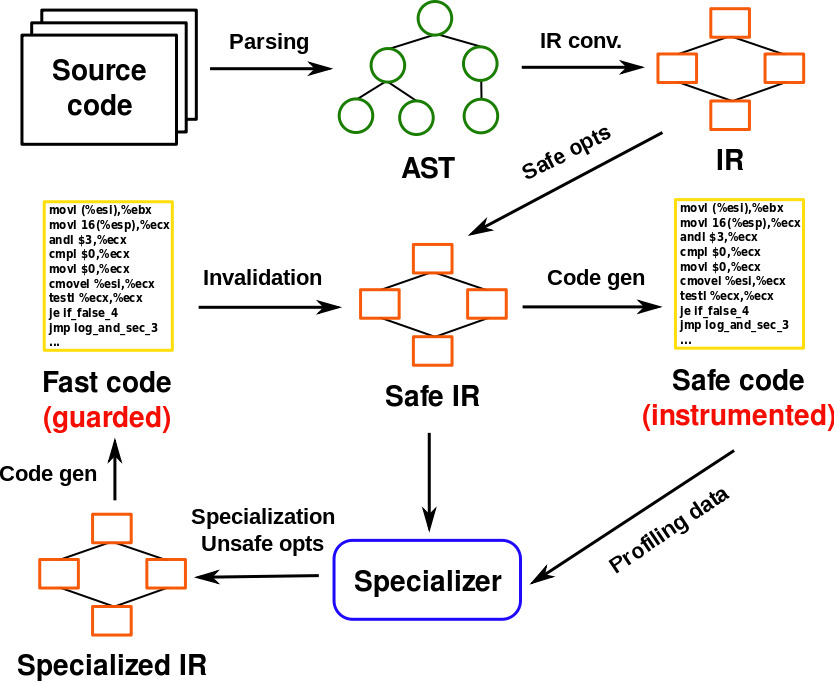
\includegraphics[width=3in]{images/transforms2}
\end{center}
\end{frame}
% ------------------------------------------------------------------------------

% -- Slide ---------------------------------------------------------------------
\begin{frame}{What Would Tachyon Do (WWTD)?}
\begin{center}
\includegraphics[height=2.8in]{images/execmodel}
\end{center}
\end{frame}
% ------------------------------------------------------------------------------

% -- Slide ---------------------------------------------------------------------
\begin{frame}{Key Ideas}
    \begin{itemize}
        \item Crucial to capture info about run time behavior
        \begin{itemize}
            \item Tracing JITs do this, but leave many run-time checks
        \end{itemize}

        \item Program needs to be correct at all times
        \begin{itemize}
            \item Don't need to run the same code at all times
            \item Multiple optimized versions correct at different times
        \end{itemize}

        \item Can make optimistic assumptions that may be invalidated
        \begin{itemize}
            \item So long as we can repair our mistakes in time
            \item Code with broken assumptions must never be executed
            \item Ideally, want invalidation to be unlikely
        \end{itemize}
    \end{itemize}
\end{frame}
% ------------------------------------------------------------------------------

% -- Slide ---------------------------------------------------------------------
\begin{frame}{Type Profiling}
    \begin{itemize}
        \item Type profiling can observe:
        \begin{itemize}
            \item Frequency of calls
            \item Types of arguments to calls
            \item Types of values stored into globals
            \item Types of values stored in object fields
        \end{itemize}

        \item Goal: build fairly accurate profile of program behavior w.r.t. types
    \end{itemize}
\end{frame}
% ------------------------------------------------------------------------------

% -- Slide ---------------------------------------------------------------------
\begin{frame}{Type Propagation}
    \begin{itemize}
        \item Form of type inference
        \item Dataflow analysis
        \item Local or whole program
        \item Rules depend on language semantics, e.g.:
        \begin{itemize}
            \item add int, int $\rightarrow$ int
            \item add float, float $\rightarrow$ float
            \item mul m4x2, m2x1 $\rightarrow$ m4x1
            \item getprop o, “a” $\rightarrow$ prop\_type(o, “a”)
        \end{itemize}

        \item In the local case, inputs are function argument types, globals types, closure variable types
        \item Output: local variable types, return type
    \end{itemize}
\end{frame}
% ------------------------------------------------------------------------------

% -- Slide ---------------------------------------------------------------------
\begin{frame}{Potential Difficulties}
    \begin{itemize}
        \item Cost of profiling
        \begin{itemize}
            \item Need accurate information
        \end{itemize}
        \item Cost of recompilation
        \begin{itemize}
            \item Usage of external threads
        \end{itemize}
        \item Frequency of recompilation
        \begin{itemize}
            \item Progressive pessimization
        \end{itemize}
        \item Inherent complexity
        \begin{itemize}
            \item Find more students!
        \end{itemize}
    \end{itemize}
\end{frame}
% ------------------------------------------------------------------------------

% -- Slide ---------------------------------------------------------------------
\begin{frame}{Related Work: Type Analysis}
    \begin{itemize}
        \item M Chevalier-Boisvert, L Hendren, C Verbrugge. \textit{Optimizing
        MATLAB through just-in-time specialization}. CC 2010.
        \item F Logozzo, H Venter. \textit{RATA: Rapid Atomic Type Analysis by
        Abstract Interpretation–Application to JavaScript Optimization}. CC
        2010.
        \item S Jensen, A M\o{}ller et al. \textit{Type analysis for JavaScript}. SAS 2009.
        \item And much more\ldots
    \end{itemize}
\end{frame}
% ------------------------------------------------------------------------------

% -- Slide ---------------------------------------------------------------------
\begin{frame}{Related work: Deoptimization}
    \begin{itemize}
        \item I Pechtchanski, V Sarkar. \textit{Dynamic optimistic
            interprocedural analysis: a framework and an application}. OOPSLA 2001.
        \begin{itemize}
            \item Systematic optimistic interprocedural type analysis to optimize polymorphic call sites
        \end{itemize}
        \item Speculative inlining
        \begin{itemize}
            \item In Java, dynamic class loading can invalidate inlining decisions
            \item Implemented in Java HotSpot VM
        \end{itemize}
        \item Polymorphic inline cache
    \end{itemize}
\end{frame}
% ------------------------------------------------------------------------------

% -- Slide ---------------------------------------------------------------------
\begin{frame}{Related Work: Tracing JITs}
    \begin{itemize}
        \item HotpathVM, TraceMonkey, LuaJIT, etc.
        \item Tracing JITs are another dynamic compilation model

        \item Same basic underlying principle
        \begin{itemize}
            \item Observe program as it runs, gather data about behavior
            \item Assume current behavior will likely persist, use data to specialize program, minimize dynamic checks
        \end{itemize}

        \item Main limitations
        \begin{itemize}
            \item Local approach, detects \& examines loops
            \item Knows little about what goes on outside loops
            \item No real way of dealing with global data, optimizing object layout, etc.
        \end{itemize}
    \end{itemize}
\end{frame}
% ------------------------------------------------------------------------------


% -- Slide ---------------------------------------------------------------------
\begin{frame}
\frametitle{\bf Distinguishing Features of Tachyon}
    \begin{itemize}
        \item Implementation flexibility
        \item Self-hosted with dynamic language
        \item Self-optimizing JIT
        \item Extensions allow using JS for stdlib (possibly even GC)
        \item Systematic optimistic optimizations
        \item Multithreaded compiler
    \end{itemize}
\end{frame}
% ------------------------------------------------------------------------------

% -- Slide ---------------------------------------------------------------------
\begin{frame}
\frametitle{\bf Ballpark Performance Comparison on \code{fib(38)}}

\begin{center}
\rowcolors{1}{RoyalBlue!10}{RoyalBlue!5}
\begin{tabular}{lll}
Tachyon     & 8.110s & (7.20x) \\
WebKit INT  & 7.334s & (6.51x) \\
WebKit      & 1.406s & (1.25x) \\
V8          & 1.127s & (1.00x) \\
gcc -O2     & 0.626s & (0.56x) \\
gcc -O3     & 0.224s & (0.20x)
\end{tabular}
\end{center}

\end{frame}
% ------------------------------------------------------------------------------

% -- Slide ---------------------------------------------------------------------
\begin{frame}
\frametitle{\bf Project Roadmap}
    \begin{enumerate}[1.]

        \item Bootstrap (March 2011)
        \begin{enumerate}[1.]
            \item Simple object representation, stdlib, FFI
            \item {\bf very few optimizations} (but careful to allow future opt)
        \end{enumerate}

        \item Competitive (September 2011)
        \begin{enumerate}[1.]
            \item GC + better object representation, full stdlib, FFI
            \item Image loader/writer
            \item Improve tools: profiler, debugger
            \item {\bf speed within factor of 2 of best JS JIT}
        \end{enumerate}

        \item Gravy (January 2012)
        \begin{enumerate}[1.]
            \item Continuations, threads
            \item Code-patching, optimistic optimizations
            \item Browser integration, real benchmarks
        \end{enumerate}

        \item Groovy (long term)
        \begin{enumerate}[1.]
            \item Persistance, contextualization
            \item On-stack replacement
        \end{enumerate}
    \end{enumerate}
\end{frame}
% ------------------------------------------------------------------------------


% -- Slide ---------------------------------------------------------------------
\begin{frame}{}
\begin{center}
{\huge\bfseries Thanks for listening!}

\vspace{5mm}%
{\large\bfseries We welcome your questions/comments}

\vspace{5mm}%
Feel free to contact the Tachyon team:\\
{\small\ttfamily \{chevalma,lavoeric,feeley,dufour\}@iro.umontreal.ca}
\end{center}
\end{frame}
% ------------------------------------------------------------------------------

\end{document}
